\subsubsection{UC10 - Informazioni dettagliate funzione}
\begin{figure}[h]
	\centering
	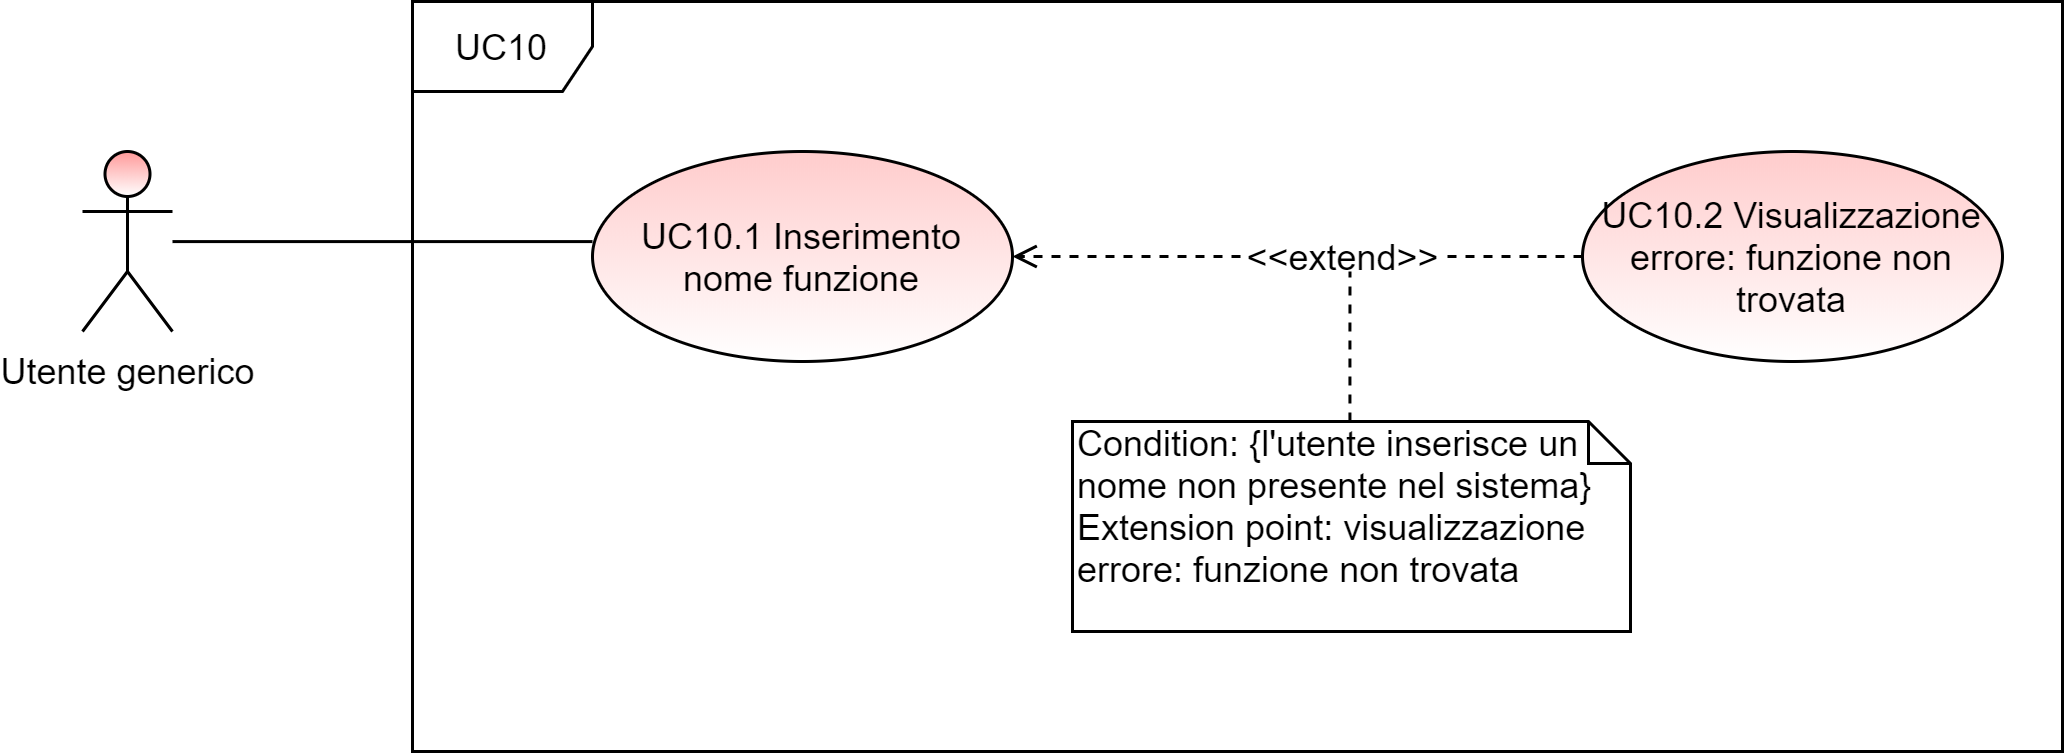
\includegraphics[scale=\ucs]{./res/img/UC10.png}
	\caption {UC10 - Informazioni dettagliate funzione}
\end{figure}
\begin{itemize}
	\item \textbf{Attori primari:} \ua{};
	\item \textbf{Attori secondari:} \re{};
	\item \textbf{Descrizione:} l’utente richiede la visualizzazione della descrizione completa di una funzione di cui conosce il nome eseguendo il comando \pinfo{}. Il sistema riporta le seguenti informazioni:  
	\begin{itemize}
		\item firma della funzione;
		\item descrizione completa della funzione.
	\end{itemize} 
	\item \textbf{Scenario principale:} 
	\begin{itemize}
		\item l'utente inserisce correttamente ed esegue il comando \pinfo{}; 
		\item vengono visualizzate le informazioni relative alla funzione in questione.
	\end{itemize}
	\item \textbf{Precondizione:} l'utente inserisce correttamente ed esegue il comando \info{};
	\item \textbf{Postcondizione:} la CLI riporta la descrizione completa della funzione in questione.
\end{itemize}